\secnumbersection{Validación de la solución} \label{section:validation}


% Se debe validar la solución propuesta. Esto significa probar o demostrar que la solución propuesta es válida para el entorno donde fue planteada.

% Tradicionalmente es una etapa crítica, pues debe comprobarse por algún medio que vuestra propuesta es básicamente válida. En el caso de un desarrollo de software es la construcción y sus pruebas; en el caso de propuestas de modelos, guías o metodologías podrían ser desde la aplicación a un caso real hasta encuestas o entrevistas con especialistas; en el caso de mejoras de procesos u optimizaciones, podría ser comparar la situación actual (previa a la memoria) con la situación final (cuando la memoria está ya implementada) en base a un conjunto cuantitativo de indicadores o criterios.

% \subsection{EJEMPLO DE COMO CITAR TABLAS}

% Se colocó una tabla que se puede referenciar también desde el texto (Ver tabla \ref{table:coloquios}).

% \begin{table}[h]
%     \centering
%     \caption{\label{table:coloquios} Coloquios del Ciclo de Charlas Informática.} Fuente: Elaboración Propia.
%     \begin{tabular}{|p{7cm}|p{7cm}|}
%         \hline
%         Título Coloquio & Presentador, País \\
%         \hline
%         ``Sensible, invisible, sometimes tolerant, heterogeneous, decentralized and interoperable... and we still need to assure its quality...''' & Guilherme Horta Travassos, Brasil.\\
%         \hline
%         ``Dispersed Multiphase Flow Modeling: From Environmental to Industrial Applications''' & Orlando Ayala, EE.UU.\\
%         \hline
%         ``Líneas de Producto Software Dinámicas para Sistemas atentos el Contexto''' & Rafael Capilla, España.\\
%         \hline
%         ... & ... \\
%         \hline
%     \end{tabular}
% \end{table}

% \subsection{Implementación}

\subsection{Stack de tecnologías}

En primera instancia existe la tentación por implementar una modificación completa de la herramienta \mesher{}, esto es viable pero se descarta cuando se prioriza la escalabilidad y mantenibilidad de código. Sobre la eficiencia y rapidez de la propuesta, que son características importantes que evidencian calidad, se evaluarán en secciones posteriores.
En \mesher{} sólo se realizarán las modificaciones descritas en las secciones anteriores que incluyen funcionalidades para identificar y exportar los Octantes a refinar, para generar estadísticas al finalizar el refinamiento en las mallas y las pequeñas modificaciones a las funcionalidades de exportación de la información de los Octantes para luego identificarlos globalmente y así refinar los Octantes correctos.

Entonces, como debemos ejecutar \mesher{}, existen varias formas de realizar esto, pero se escogerá la que utilice menos recursos para ejecutar llamadas a sistema como lo hace \textit{bash} en linux. Ya que se requiere de funcionalidades básicas como iteraciones y manipulación de archivos, esta es una buena herramienta a utilizar.

\subsection{Proceso de análisis}

Para validar la propuesta, se utilizará una serie de mallas con diferentes complejidades.
\begin{itemize}
    \item Malla de corteza cerebral con área de refinamiento prismática en la zona frontal.

        Propuesta inicial, de por sí la malla de corteza cerebral posee una complejidad media, contiene algunas zonas cóncavas que podrían enriquecer la validación del algoritmo. El prisma se posicionará en la zona del lóbulo frontal.
    \item Malla de corteza cerebral con área de refinamiento prismática en la zona trasera.

        En la zona trasera, lóbulo occipital de la corteza cerebral, de naturaleza cóncava e irregular se posicionará el prisma para refinar localmente, esto con el fin de complejizar el trabajo del algoritmo.
    \item Malla de Moai con área de refinamiento prismática en la zona superior.

        Para este análisis se escogió una representación de un Moai, que naturalmente no posee múltiples zonas cóncavas, entonces se aplicará el área de refinamiento en la zona superior donde se presenta la mayor cantidad de zonas cóncavas. 
    \item Malla de Moai con área de refinamiento prismática en la zona inferior.

        Se utilizará también la zona inferior, que no posee mayor nivel de complejidad respecto a su concavidad, con motivo de aumentar el universo de soluciones.
    \item Malla de paladar con área de refinamiento prismática en la zona superior.

        Esta representación posee áreas muy finas con respecto al resto de la malla, entonces se aplicó un área de refinamiento adicional en la zona superior por su complejidad en función de concavidad.
    \item Malla de coxis.

        En general esta representación es muy compleja, presenta zonas muy pequeñas y con múltiples concavidades.
\end{itemize}

Luego de realizar algunas iteraciones básicas para tener una idea del comportamiento del algoritmo con las mallas, realizando iteraciones donde se añadieron áreas prismáticas en diferentes zonas y otras iteraciones donde se modificaron los niveles de refinamiento tanto general como del área prismática

Se identificaron dos factores importantes para tratar cada malla, y que si bien, parecen tener una correlación, este trabajo no busca encontrar dicha relación, por tanto, se supondrán como factores sin correlación.
\begin{itemize}
	\item Complejidad geométrica
		Algunas mallas se notaron con alta densidad de regiones que forman depresiones o concavidades. Incluso algunas de ellas, presentaban alta densidad de estas zonas sólo en cierta parte de la representación.
		Entonces para aquellas que presentaban su alta densidad de concavidades en una área determinada, se le aplicó el área prismática tanto en su zona de alta densidad como también fuera de ella, como sucede en el caso de la representación del Moai y Corteza Cerebral.
		Para otras mallas, simplemente se insertó un área prismática con el fin de generar \elements{} inválidos, como sucede en el Paladar, que si bien, presenta variedad de zonas cóncavas, no genera \elements{} inválidos con sólo refinar globalmente, entonces para este caso, se realizaron variaciones en su refinamiento global presentando sólo una opción de posición en su zona prismática de refinamiento local.
		
	\item Capacidad Computacional
		Esto hace alusión principalmente al tiempo que demora el algoritmo en realizar refinamiento global o incluso mallas que generan detenimientos forzados del proceso donde se ejecuta el algoritmo por, quizás, presentar un alto número de vértices y aristas, tan alta que el sistema operativo probablemente queda sin memoria. Como por ejemplo, cuando se realizó un refinamiento global de nivel nueve en la malla del Coxis.
\end{itemize}

Luego de iterar las mallas, se analizará sus estadísticas sobre \elements{} de mala calidad.

\subsection{Ejecución}

En cada malla dependiendo de su complejidad se aplicará o no, un área prismática para refinar localmente, de esta manera añadir consistencia a los resultados.

La única malla a la que no se le aplicará el área prismática es la malla de coxis debido a su compleja naturaleza explicada en el itemizado anterior.

A cada caso, se ejecutará el algoritmo con threshold $t \in \{ 0, 0.03, 0.05 \}$ y debido a que $E$ en la mayoría de los casos converge evidentemente en las primeras diez iteraciones, se escoge esta como cota superior.

Es necesario, antes de comenzar, definir lo siguiente. Se referirá a una malla con refinamiento global de nivel $X$ y refinamiento local de nivel $Y$, como la malla $XrY$.

Entonces una ejecución del algoritmo para la corteza cerebral con $RL_{global}=5$, $RL_{local}=7$, región prismática con identificador $2$, número de iteración $5$ y threshold $0.03$,  se expondrá como ``cortex\_3\_5r7\_1\_n'', teniendo la siguiente estructura ``<malla\_threshold\_$RL_{global}$r$RL_{local}$\_$ROI_{id}$\_iteración>''.

\subsubsection{Malla de corteza cerebral}

La corteza cerebral, si bien, presenta amplias zonas irregulares, el algoritmo no presenta problemas en su ejecución. Entonces se tratará como un caso para analizar complejidad geométrica.

Al implementar el algoritmo propuesto en la malla de corteza cerebral, entregándole como input las cotas definidas recientemente, el modelo de la corteza, los modelos de la superficie prismática a refinar, la base de nombre de los archivos exportados y una cota de diez iteraciones.  Obtenemos los siguientes resultados \autoref{fig:bar_cortex_all}, que nos muestra un histograma agrupado por los primeros cuatro intervalos de calidad.

En la parte superior del recuadro, se muestran los histogramas para la primera superficie y en la parte inferior para la segunda superficie, frontal y occipital respectivamente, en la \autopageref{fig:c_5r7_all} se evidencia la disposición de las superficies en la corteza.


\begin{figure}[!ht]
    \centering
    \begin{subfigure}[t]{0.45\textwidth}
        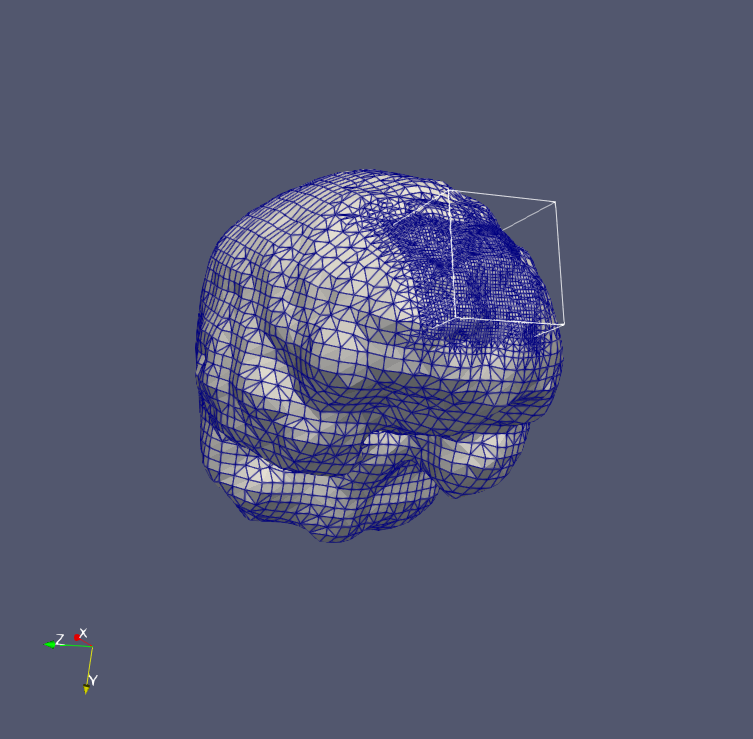
\includegraphics[width=1.0\textwidth]{figures/meshes/c_5r7_01.png}
        \caption{Representación corteza cerebral con refinamiento en lóbulo frontal.}
    \end{subfigure}
    \begin{subfigure}[t]{0.45\textwidth}
        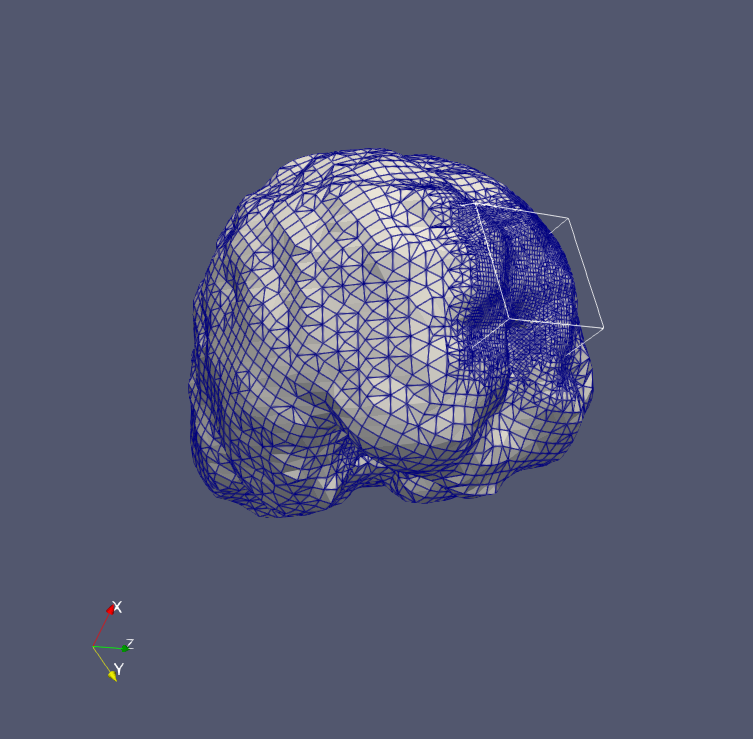
\includegraphics[width=1.0\textwidth]{figures/meshes/c_5r7_2_01.png}
        \caption{Representación corteza cerebral con refinamiento en lóbulo occipital.}
    \end{subfigure}
    \caption{ Diferentes localidades de refinamiento en corteza cerebral. }
    Fuente: Elaboración propia.
    \label{fig:c_5r7_all}
\end{figure}


\subsubsection{Malla de Moai}

La ejecución del algoritmo en la malla de Moai para los casos con refinamiento inferior y superior, como podemos ver dispuestas en \autoref{fig:moai_5r7_all}, la superficie de la zona inferior se identificará como la superficie 1 y la superior se identificará como la malla 2. Se puede ver claramente la diferencia en la complejidad geométrica entre ambas superficies, teniendo en la parte superior más concavidades relacionadas a las facciones del moai. Luego, en \autoref{fig:bar_moai_all}, se puede identificar claramente, cómo la superficie 1 se muestra más simple, reduciendo considerablemente más rápido la cantidad de \elements{} de mala calidad en pocas iteraciones.
No así en la superficies superior, dónde se puede notar como en las primeras iteraciones, para todos los thresholds aumenta en su segunda iteración la cantidad de \elements{} negativos.

en \autoref{fig:bar_moai_all}. 

\begin{figure}[!ht]
    \centering
    \begin{subfigure}[t]{0.45\textwidth}
        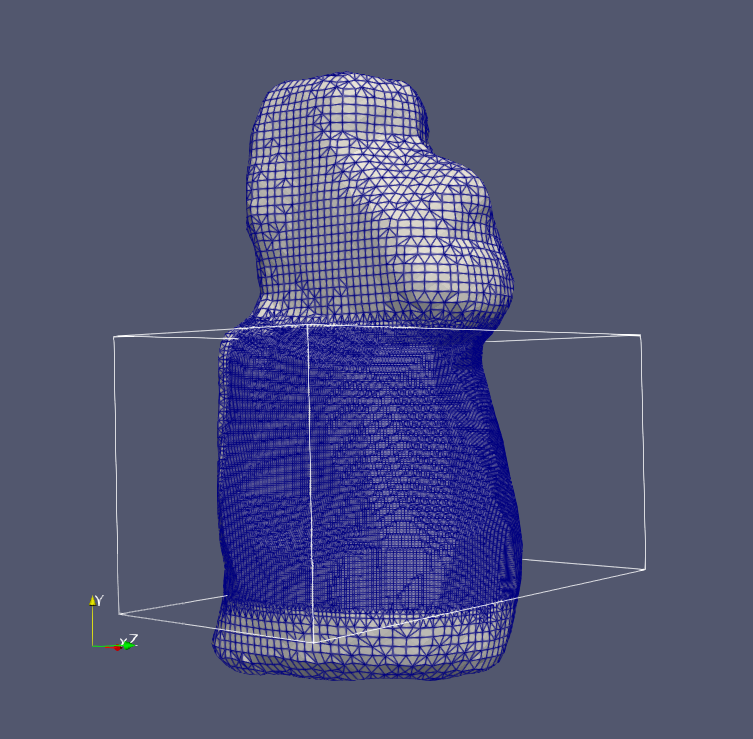
\includegraphics[width=1.0\textwidth]{figures/meshes/moai_5r7_01.png}
        \caption{Representación Moai con refinamiento en zona inferior.}
    \end{subfigure}
    \begin{subfigure}[t]{0.45\textwidth}
        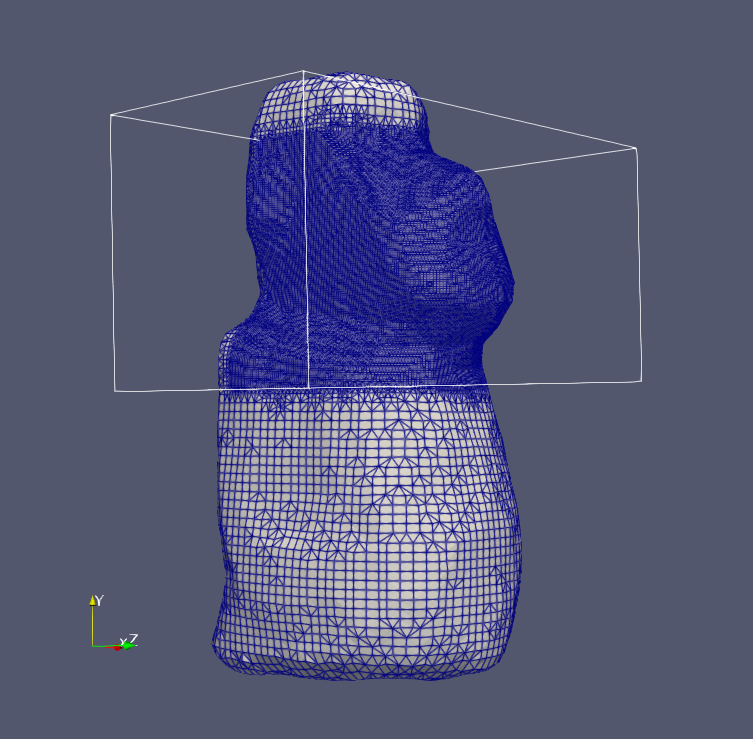
\includegraphics[width=1.0\textwidth]{figures/meshes/moai_5r7_2_01.png}
        \caption{ Representación Moai con refinamiento en zona superior. }
    \end{subfigure}
    \caption{ Diferentes localidades de refinamiento en Moai. }
    Fuente: Elaboración propia.
    \label{fig:moai_5r7_all}
\end{figure}

\subsubsection{Malla de paladar}

En el caso de la malla de paladar, se realizó un refinamiento general de nivel 5 y 6, que no generó \elements{} inválidos, por tanto, se trabajará sólo con un área prismática ubicada en la zona superior por su alta densidad de zonas cóncavas, como en \autoref{fig:palate_5r7_all}. 

Como se muestra en \autoref{fig:bar_palate_all} los resultados, todas las instancias lograron ``mallas solución'' en por lo menos 6 iteraciones.

\begin{figure}[!ht]
    \centering
    \begin{subfigure}[t]{0.8\textwidth}
        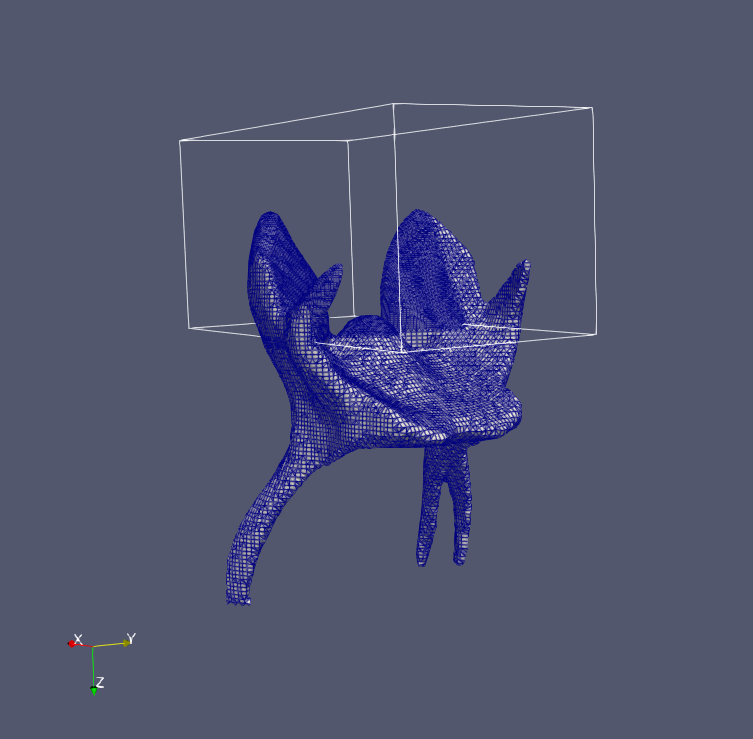
\includegraphics[width=1.0\textwidth]{figures/meshes/palate_5r7_01.png}
        % \caption{Representación Paladar con refinamiento en zona superior.}
    \end{subfigure}
    \caption{ Representación Paladar con refinamiento en zona superior. }
    Fuente: Elaboración propia.
    \label{fig:palate_5r7_all}
\end{figure}

\subsubsection{Malla de coxis}

Para la representación del Coxis, inicialmente no se utilizó una zona de refinamiento adicional al comienzo de las pruebas porque como se muestra en la \autoref{fig:coxis_8r9_all}, es evidente la amplia densidad de Elementos y concavidades en la malla. Esto genera Elementos inválidos sólo aplicando el algoritmo de generación mallas. Entonces, se escogieron niveles de refinamiento global que permitieran ejecutar el algoritmo de forma eficaz, esto es entre los niveles 4 y 9, el nivel cuatro se escogió porque genera una malla con elemento inválidos pero al momento de visualizarla genera una representación con falta de detalle, no representa muy bien la realidad. El nivel nueve se escogió como cota superior porque genera un error en el sistema debido al alto número de nodos en la malla.

Para esta sección de la validación entonces se utilizaron los niveles 5 y 8 como cotas superior e inferior y se definieron dos casos con refinamiento global y local para una superficie prismática ubicada en la parte superior de la cadera, y tres casos con refinamiento global solamente, describiéndolas respectivamente como $4r7$, $5r8$ y $6$,$7$ y $8$

%Luego, como se evidenciará más adelante, en el análisis de los resultados, se puede ver claramente que el algoritmo diverge en cuanto a frecuencia de elementos inválidos. Es por esto que para esta sección de la validación, donde se realizó refinamiento global y local, se orientó el estudio en encontrar una relación entre la cantidad de elementos inválidos y la diferencia entre los niveles de refinamiento.


Es necesario mencionar, que se realizaron pruebas con los casos $6r8$ y $5r9$, pero no generaron una ejecución válida del algoritmo.
Además, se colorearon los \octants{} a refinar en cada iteración y siempre mostraban presencia en las articulaciones de la cadera y columna, zonas bastante pequeñas para el alcance de los niveles de refinamiento.


\begin{figure}[!ht]
    \centering
    \begin{subfigure}[t]{0.8\textwidth}
        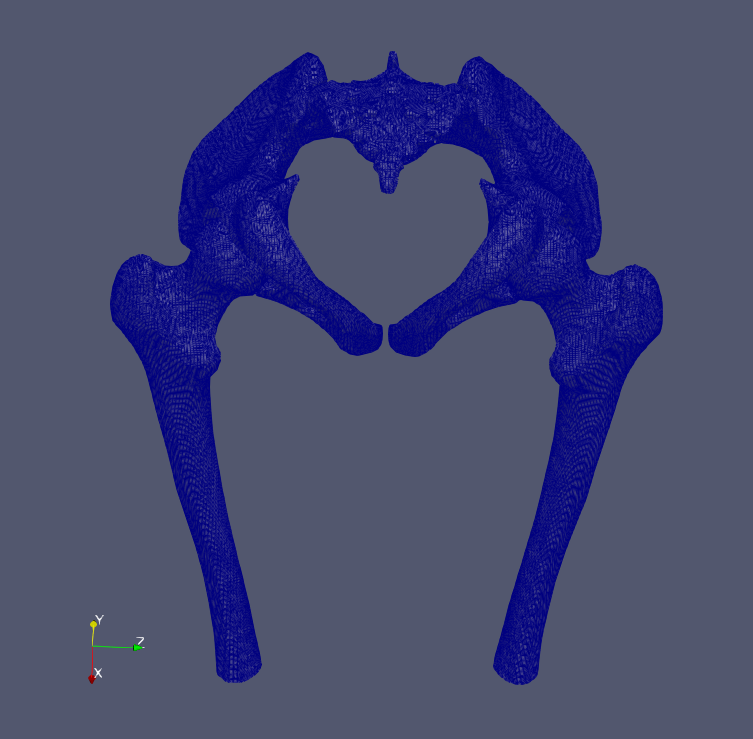
\includegraphics[width=1.0\textwidth]{figures/meshes/coxis_8r9_01.png}
    \end{subfigure}
    \caption{ Representación Coxis sin refinamiento local. }
    Fuente: Elaboración propia.
    \label{fig:coxis_8r9_all}
\end{figure}


Es incluso una malla interesante de analizar, se logró mallas con diversos niveles de refinamiento. Niveles seis, siete, ocho y nueve de refinamiento global, además de agregar una sección prismática en las zona superior del coxis, cubriendo por completo las zonas más pequeñas de la malla, en ningún caso se logró la convergencia del algoritmo.


%Este caso, se probó aplicando menor $rl$ global y una zona prismática en una de las articulaciones y se mantiene constante la cantidad de elementos inválidos, aproximadamente $E_0 = 45$.



\subsection{Resultados}

Para analizar el comportamiento del algoritmo, nos enfocaremos en ajustar la frecuencia de Elementos inválidos a algún modelo conocido, entregar una hipótesis sobre la anomalía en la malla del Coxis y comparar con los resultados entregados en \cite{daines2018repairing}.

\subsubsection{Ajuste de la cantidad de iteraciones}

El algoritmo propuesto se comporta de muy buena manera para todas las mallas a excepción de la que representa el Coxis.  Cuando el algoritmo logra converger en una malla válida, es posible reducir considerablemente la cantidad de Octantes por refinar a lo más diez iteraciones, a simple vista se podría entregar una hipótesis sobre el comportamiento del algoritmo en cada iteración.

Para esto, se considerará, a diferencia de lo que ya es tónica en lo antes mostrado, la frecuencia de Elementos que cumplen ciertas condiciones respecto a su calidad, para referirse a la frecuencia de Elementos, se denotará como $E$. Luego, para el análisis sobre ajuste del comportamiento del algoritmo, se considerará, la frecuencia de todos los Elementos que pertenecen a la malla y tienen $J_{ENS} \leq 0$, esto será $E^0$. 

Se elaboró la siguiente tabla con el $E^0$ en cada iteración para las diferentes mallas de los casos definidos, \autoref{table:num_els_ref}. Lo evidente es la relación estrecha entre Elementos y Octantes, dicho comportamiento se respalda en su naturaleza estructural. Luego, la aparente relación en el comportamiento de $E$ en todos los casos, permite comenzar la búsqueda del modelo, por uno exponencial.


En la \autoref{table:num_els_ref} se muestra el comportamiento de $E^0$ en cada iteración, de aquí solamente se analizarán los casos que convergen a cero.

\begin{table}[!ht]
\begin{tabular}{|lllllll|}
\hline
\multicolumn{7}{|c|}{Número de Elementos por refinar en cada iteración.}                                                                                                                                                                                                                    \\ \hline
\multicolumn{1}{|l|}{\textbf{N° Iteración}} & \multicolumn{1}{l|}{\textbf{cortex\_5r7}} & \multicolumn{1}{l|}{\textbf{cortex\_5r7\_2}} & \multicolumn{1}{l|}{\textbf{moai\_5r7}} & \multicolumn{1}{l|}{\textbf{moai\_5r7}} & \multicolumn{1}{l|}{\textbf{palate\_6r7}} & \textbf{coxis\_7} \\ \hline
\multicolumn{1}{|l|}{1}                     & \multicolumn{1}{l|}{27}                   & \multicolumn{1}{l|}{64}                      & \multicolumn{1}{l|}{26}                 & \multicolumn{1}{l|}{15}                 & \multicolumn{1}{l|}{25}                   & 242               \\ \hline
\multicolumn{1}{|l|}{2}                     & \multicolumn{1}{l|}{7}                    & \multicolumn{1}{l|}{32}                      & \multicolumn{1}{l|}{7}                  & \multicolumn{1}{l|}{12}                 & \multicolumn{1}{l|}{5}                    & 658               \\ \hline
\multicolumn{1}{|l|}{3}                     & \multicolumn{1}{l|}{2}                    & \multicolumn{1}{l|}{13}                      & \multicolumn{1}{l|}{2}                  & \multicolumn{1}{l|}{11}                 & \multicolumn{1}{l|}{3}                    & 435               \\ \hline
\multicolumn{1}{|l|}{4}                     & \multicolumn{1}{l|}{1}                    & \multicolumn{1}{l|}{6}                       & \multicolumn{1}{l|}{1}                  & \multicolumn{1}{l|}{3}                  & \multicolumn{1}{l|}{1}                    & 612               \\ \hline
\multicolumn{1}{|l|}{5}                     & \multicolumn{1}{l|}{0}                    & \multicolumn{1}{l|}{7}                       & \multicolumn{1}{l|}{1}                  & \multicolumn{1}{l|}{0}                  & \multicolumn{1}{l|}{1}                    & 679               \\ \hline
\multicolumn{1}{|l|}{6}                     & \multicolumn{1}{l|}{}                     & \multicolumn{1}{l|}{3}                       & \multicolumn{1}{l|}{0}                  & \multicolumn{1}{l|}{}                   & \multicolumn{1}{l|}{0}                    & 746               \\ \hline
\multicolumn{1}{|l|}{7}                     & \multicolumn{1}{l|}{}                     & \multicolumn{1}{l|}{0}                       & \multicolumn{1}{l|}{}                   & \multicolumn{1}{l|}{}                   & \multicolumn{1}{l|}{}                     & 880               \\ \hline
\multicolumn{1}{|l|}{8}                     & \multicolumn{1}{l|}{}                     & \multicolumn{1}{l|}{}                        & \multicolumn{1}{l|}{}                   & \multicolumn{1}{l|}{}                   & \multicolumn{1}{l|}{}                     & 1017              \\ \hline
\multicolumn{1}{|l|}{9}                     & \multicolumn{1}{l|}{}                     & \multicolumn{1}{l|}{}                        & \multicolumn{1}{l|}{}                   & \multicolumn{1}{l|}{}                   & \multicolumn{1}{l|}{}                     & 1179              \\ \hline
\multicolumn{1}{|l|}{10}                    & \multicolumn{1}{l|}{}                     & \multicolumn{1}{l|}{}                        & \multicolumn{1}{l|}{}                   & \multicolumn{1}{l|}{}                   & \multicolumn{1}{l|}{}                     & 1302              \\ \hline
\end{tabular}
\caption{ $E^0$ en cada iteración para los diferentes casos. }
\label{table:num_els_ref}
\end{table}

\subsection{Análisis de los resultados}


\subsubsection{ Análisis de la tasa de reducción de la cantidad de Elementos por refinar en cada iteración }

\begin{itemize}
    \item Definición de una secuencia exponencial.

    Para determinar si $E$ se comporta de manera exponencial, es esencial revisar cómo se comportan las reducciones entre cada par de números consecutivos y si sigue un patrón consistente con un modelo exponencial.

    Un modelo exponencial sigue la forma:
    $$y = a \cdot r^n$$
     
    donde:
    
    \begin{itemize}
        \item y es el valor en la n-ésima posición.
        \item a es el valor inicial (en nuestro caso, 21).
        \item r es la razón de reducción (un valor menor a 1).
        \item n es la posición en la secuencia.
    \end{itemize}
    
    Para verificar si una secuencia sigue un modelo exponencial, podemos examinar si el cociente entre cada par de términos consecutivos es aproximadamente constante. Es decir, si $\frac{y_{n+1}}{y_n}$ es constante.

    \item Cálculo del cociente entre términos consecutivos

    Calculamos el cociente entre cada par de números consecutivos en la secuencia de cada uno de los casos. \autoref{table:co_els_ref}

	\begin{table}[!ht]
	\centering
	\begin{tabular}{|llllll|}
	\hline
	\multicolumn{6}{|c|}{ Cociente entre cantidad de Elementos por refinar consecutivos}                                                                                                                                                                           \\ \hline
	\multicolumn{1}{|l|}{\textbf{N° Iteración}} & \multicolumn{1}{l|}{\textbf{cortex\_5r7}} & \multicolumn{1}{l|}{\textbf{cortex\_5r7\_2}} & \multicolumn{1}{l|}{\textbf{moai\_5r7}} & \multicolumn{1}{l|}{\textbf{moai\_5r7}} & \textbf{palate\_6r7} \\ \hline
	\multicolumn{1}{|l|}{1-2}                   & \multicolumn{1}{l|}{0.259}          & \multicolumn{1}{l|}{0.500}             & \multicolumn{1}{l|}{0.269}         & \multicolumn{1}{l|}{1.25}         & 0.2             \\ \hline
	\multicolumn{1}{|l|}{2-3}                   & \multicolumn{1}{l|}{0.286}            & \multicolumn{1}{l|}{0.406}             & \multicolumn{1}{l|}{0.285}          & \multicolumn{1}{l|}{0.733}        & 0.6              \\ \hline
	\multicolumn{1}{|l|}{3-4}                   & \multicolumn{1}{l|}{0.500}            & \multicolumn{1}{l|}{0.462}              & \multicolumn{1}{l|}{0.5}            & \multicolumn{1}{l|}{0.273}         & 0.333            \\ \hline
	\multicolumn{1}{|l|}{4-5}                   & \multicolumn{1}{l|}{}                     & \multicolumn{1}{l|}{1.166}               & \multicolumn{1}{l|}{1.0}            & \multicolumn{1}{l|}{}                   & 1.0              \\ \hline
	\multicolumn{1}{|l|}{5-6}                   & \multicolumn{1}{l|}{}                     & \multicolumn{1}{l|}{0.429}               & \multicolumn{1}{l|}{}                   & \multicolumn{1}{l|}{}                   &                      \\ \hline
	\end{tabular}
	\caption{Cocientes entre cantidades de Elementos con $J_{ENS} \leq 0$ para los diferentes casos. }
	\label{table:co_els_ref}
	\end{table}


    \item Evaluación de los Cocientes.

    Para un modelo exponencial puro, los cocientes entre términos consecutivos deberán ser aproximadamente iguales. En este caso, los valores no lo son, pero están en un rango que sugiere una tendencia decreciente. Sin embargo, la variabilidad entre los cocientes da indicios de que la secuencia no se reduce de manera perfectamente exponencial con una sola razón común.

	Por ejemplo, en el caso de \textit{cortex\_5r7\_2}, sus cocientes se mantienen relativamente constante, aproximadamente $0.45$, a excepción del cociente en las iteraciones \textit{4-5} que se escapa casi al doble del promedio.


    \item Ajuste a un modelo exponencial

	Se ajustará a un modelo exponencial cada uno de los casos. Considerando $a_i$, valor inicial del caso $i$, se buscará una razón $r_i$ que mejor ajuste la reducción de la secuencia para el caso.
    
    Para esto, es necesario resolver la ecuación $$y = a_i \cdot r_{i}^{n}$$ para cada $n$ y encontrar el $r_i$ promedio que mejor describa la secuencia. Aunque los cocientes no son constantes, podemos ver si hay un $\bar{r_i}$ promedio que se ajuste razonablemente.

    \item Cálculo promedio geométrico

    El promedio geométrico de los cocientes es una manera de obtener una aproximación de la razón $\bar{r_i}$:

    Su valor se calcula en \autoref{table:r_fit}.

	\begin{table}[!ht]
 		\centering
		\begin{tabular}{|ll|}
		\hline
		\multicolumn{2}{|c|}{Promedio geométrico de los cocientes de cada caso}     \\ \hline
		\multicolumn{1}{|l|}{\textbf{Casos} $\mathbf{i}$}     & Promedio geométrico $\mathbf{\bar{r_i}}$ \\ \hline
		\multicolumn{1}{|l|}{cortex\_5r7}    & 0.333                                \\ \hline
		\multicolumn{1}{|l|}{cortex\_5r7\_2} & 0.542                                \\ \hline
		\multicolumn{1}{|l|}{moai\_5r7}      & 0.443                                \\ \hline
		\multicolumn{1}{|l|}{moai\_5r7\_2}   & 0.630                                \\ \hline
		\multicolumn{1}{|l|}{palate\_6r7}    & 0.408                                \\ \hline
		\end{tabular}
		\caption{Promedio geométrico de los cocientes de cada caso. }
		\label{table:r_fit}
	\end{table}

    Estos $\bar{r_i}$ indican que las secuencias podrían ajustarse aproximadamente por un modelo exponencial con razones cercanas a las propuestas en la tabla \ref{table:r_fit}.

    Gráficamente podemos ver el comportamiento de $E^0$ en cada iteración sobre los datos reales en \autoref{fig:exponential_fit_all}.  La gran mayoría de los casos se ajustan de buena manera, podríamos decir que el algoritmo se comporta bajo un modelo exponencial, sin considerar el caso excepcional del coxis.  A diferencia de los demás casos, la malla del coxis diverge también de manera exponencial.  Esto puede explicarse debido al comportamiento en cascada que tiene el algoritmo y la estructura continua de las vecindades cóncavas.
    
%	\begin{figure}[!ht]
%		\centering
%		\begin{subfigure}[t]{0.49\textwidth}
%			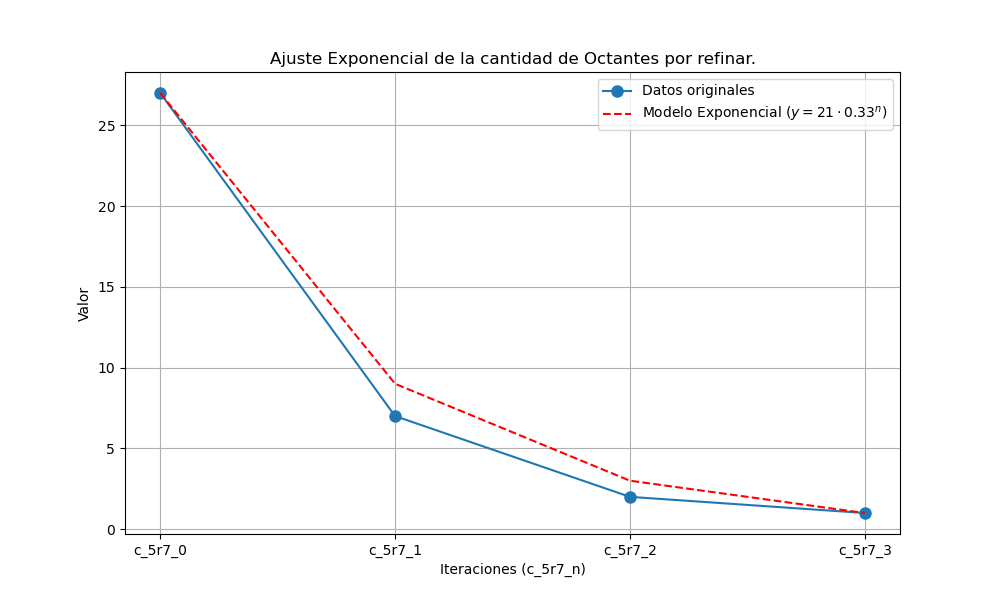
\includegraphics[width=1.0\textwidth]{figures/analysis/cortex/c_5r7_1_fit.png}
%		\end{subfigure}
%		\hfill
%		 \begin{subfigure}[t]{0.49\textwidth}
%			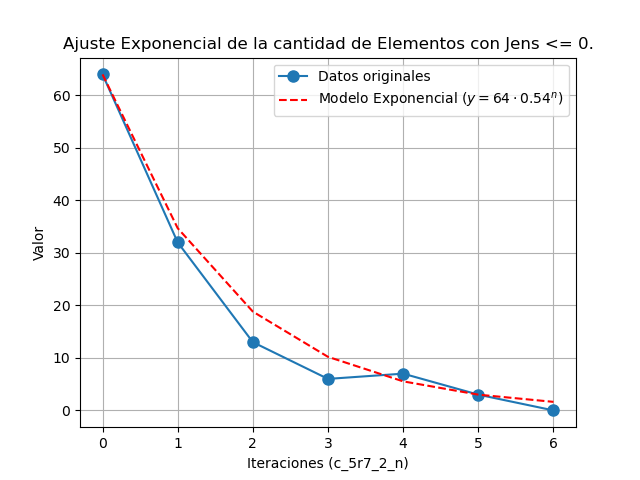
\includegraphics[width=1.0\textwidth]{figures/analysis/cortex/c_5r7_2_2_fit.png}
%		\end{subfigure}
%		\hfill
%		\begin{subfigure}[t]{0.49\textwidth}
%			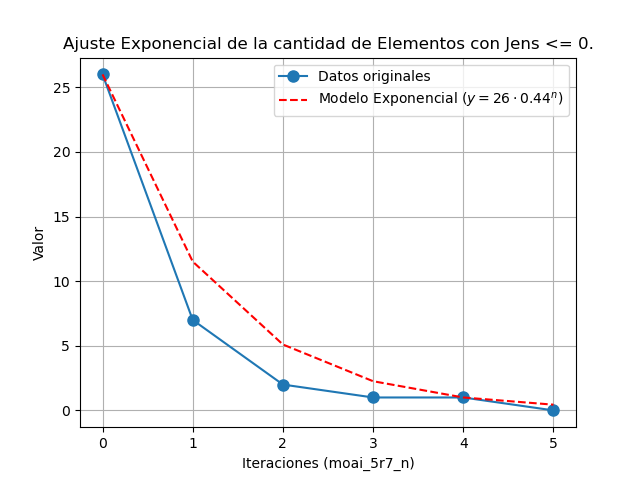
\includegraphics[width=1.0\textwidth]{figures/analysis/moai/moai_5r7_1_fit.png}
%		\end{subfigure}
%		\hfill
%		\begin{subfigure}[t]{0.49\textwidth}
%			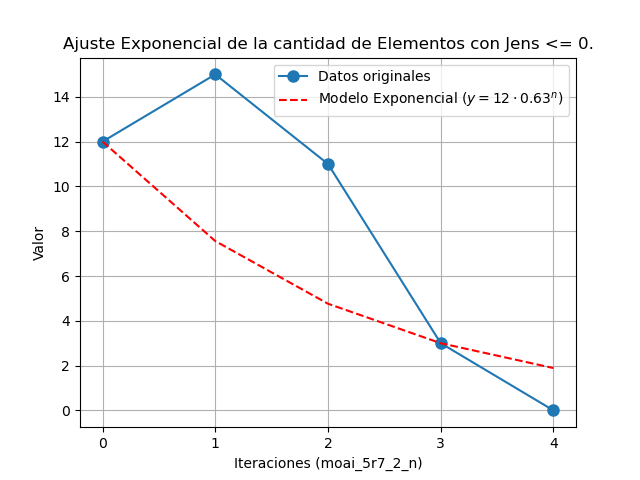
\includegraphics[width=1.0\textwidth]{figures/analysis/moai/moai_5r7_2_2_fit.png}
%		\end{subfigure}
%		\hfill
%		\begin{subfigure}[t]{0.49\textwidth}
%			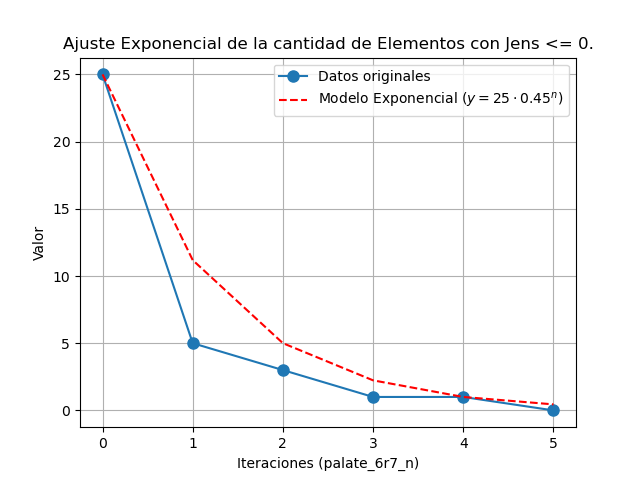
\includegraphics[width=1.0\textwidth]{figures/analysis/palate/palate_6r7_1_fit.png}
%		\end{subfigure}
%		\hfill
%		\begin{subfigure}[t]{0.49\textwidth}
%		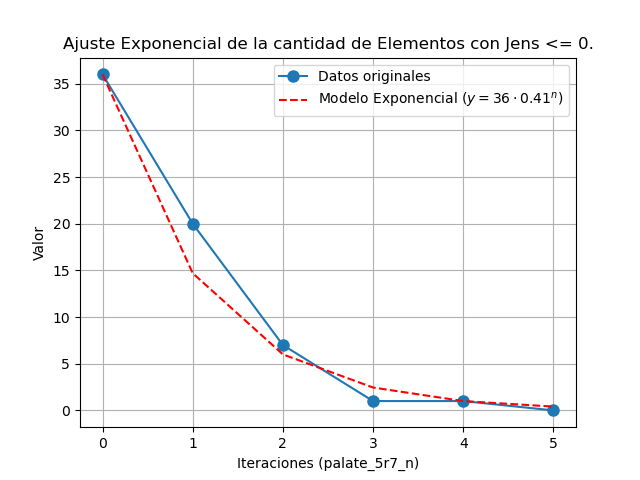
\includegraphics[width=1.0\textwidth]{figures/analysis/palate/palate_5r7_1_fit.png}
%		\end{subfigure}
%	\end{figure}
%		
%	\begin{figure}[!ht]
%		\ContinuedFloat
%		\centering
%		\begin{subfigure}[t]{0.49\textwidth}
%		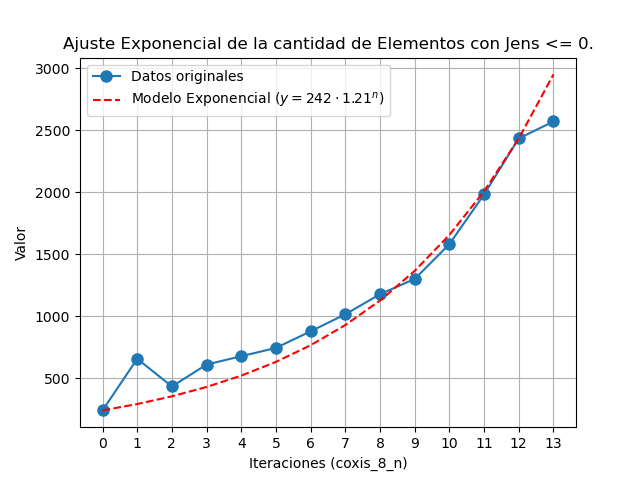
\includegraphics[width=1.0\textwidth]{figures/analysis/coxis/coxis_8_1_fit.png}
%		\end{subfigure}
%		\caption{ Representación Coxis sin refinamiento local. }
%		Fuente: Elaboración propia.
%		\label{fig:exponential_fit_all}
%	\end{figure}


	\begin{figure}[!ht]
		\centering
		\begin{subfigure}[t]{1.0\textwidth}
			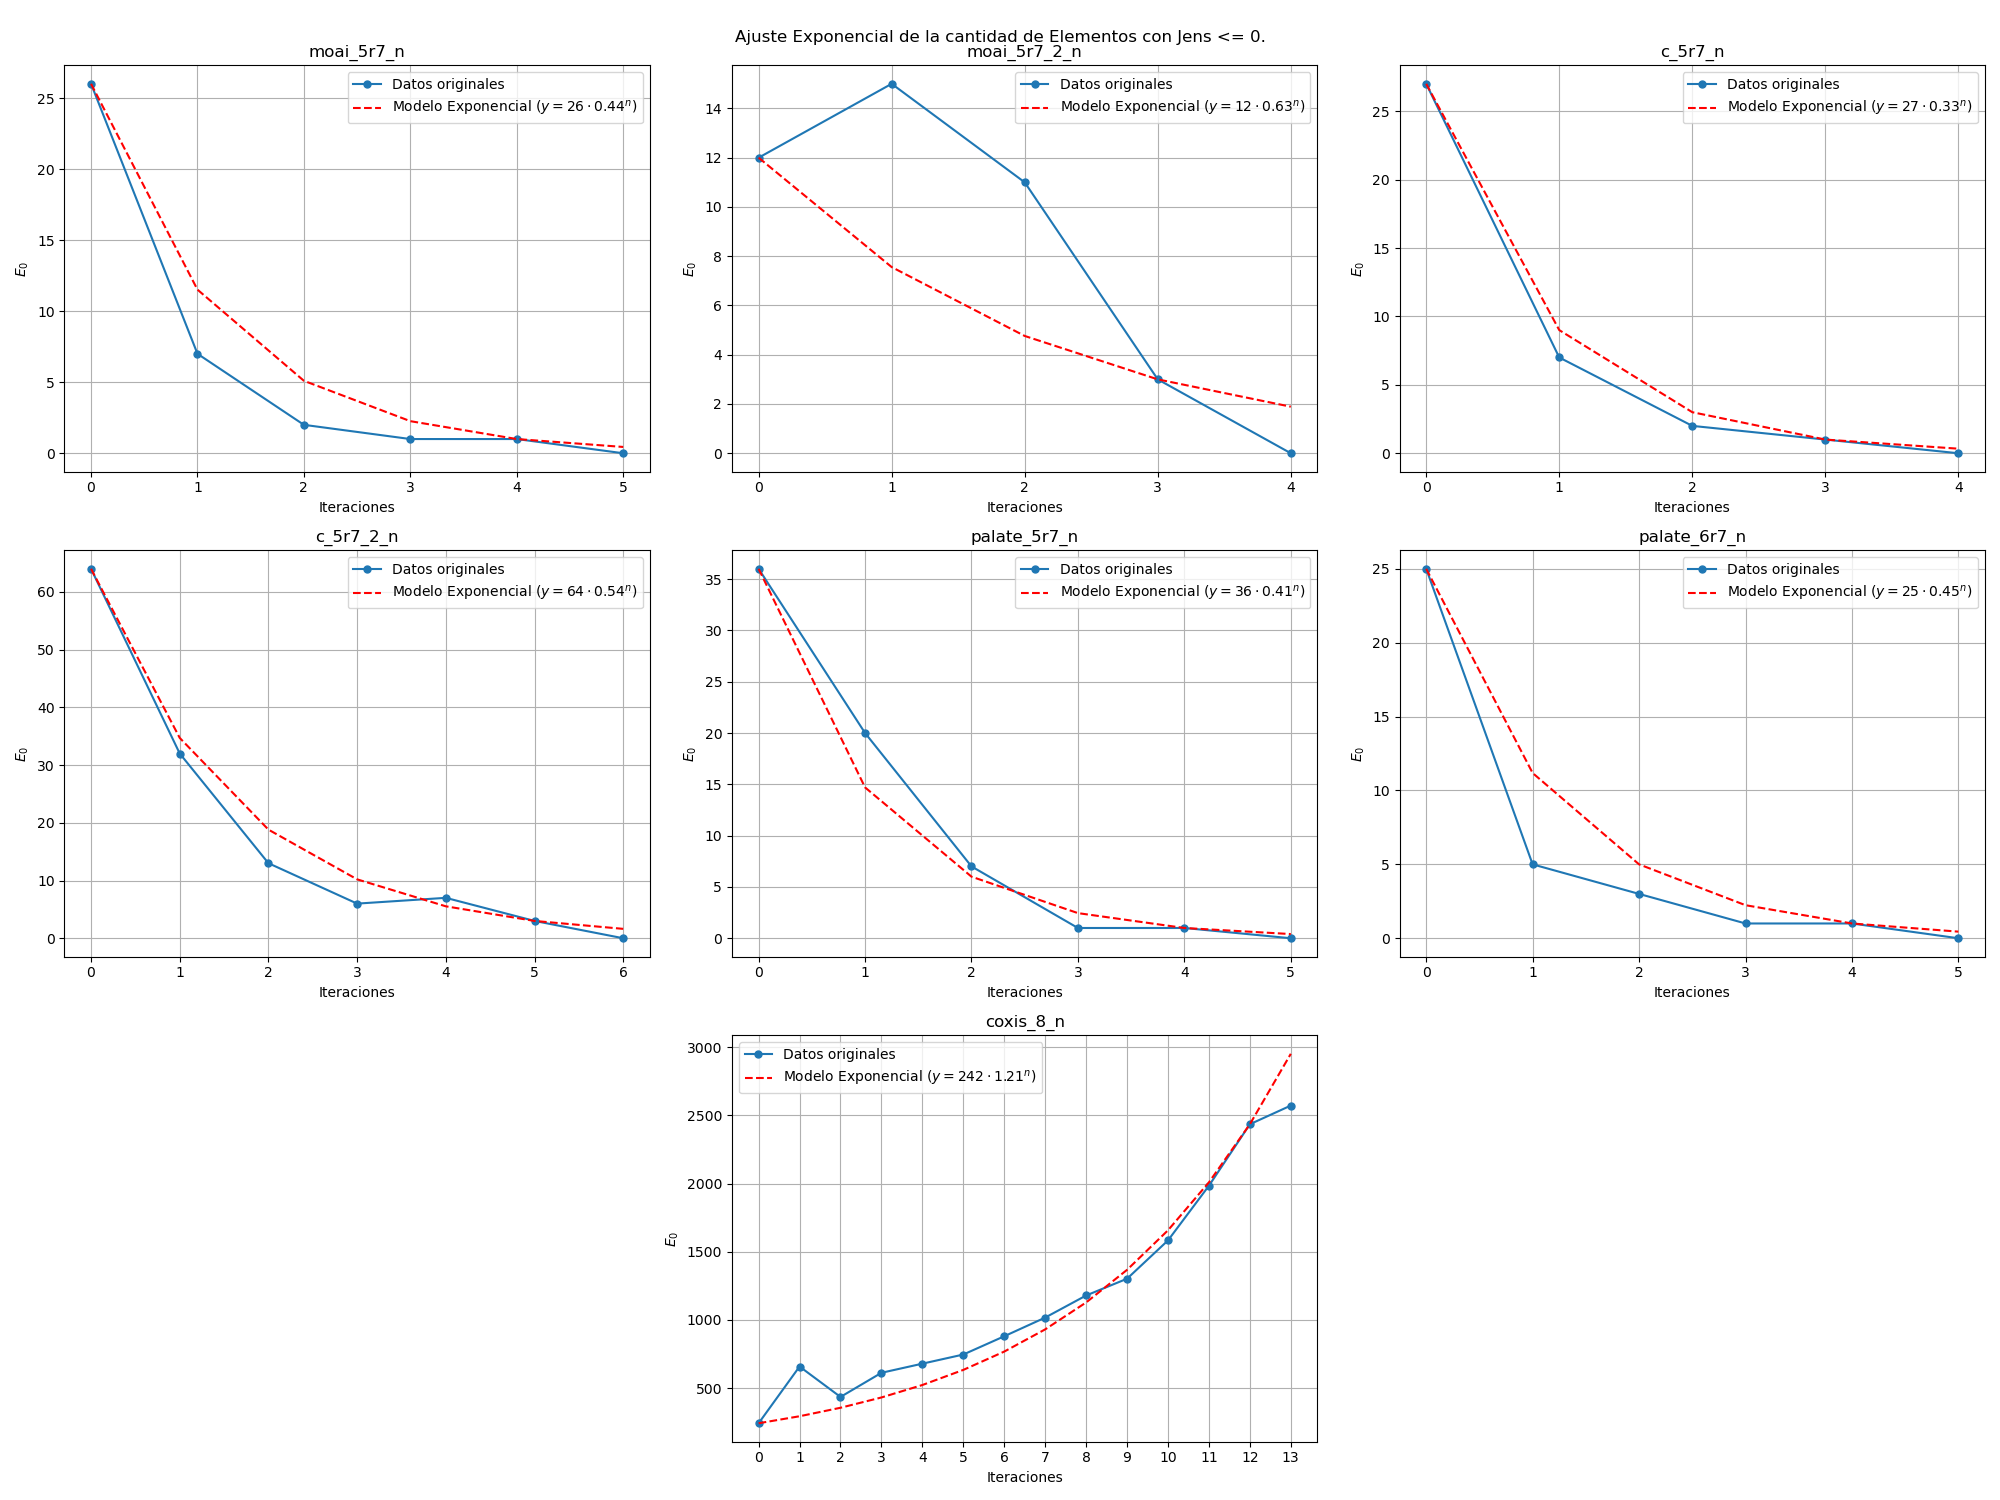
\includegraphics[width=0.75\paperheight, angle=90, origin=c]{figures/analysis/fit_all.png}
		\end{subfigure}
		\caption{ Ajuste exponencial de $E^0$ para todos los casos. }
		Fuente: Elaboración propia.
		\label{fig:exponential_fit_all}
	\end{figure}

\end{itemize}


%\breakpoint{Comienzo 11-08-2024}

\subsubsection{ Análisis del efecto en los Elementos adyacentes }

Cuando se refina cada Octante con Elementos inválidos, genera una reacción en cadena de refinamiento en los Octantes adyacentes para mantener la consistencia en los niveles de refinamiento de la malla. Debe cumplirse que, dado un Octante Objetivo $O$ con nivel de refinamiento $rl_o$, deben, sus vecinos directos, $\bar{O}$, tener un nivel de refinamiento $rl_{\bar{o}} \in \{rl_o + 1, rl_o - 1, rl_o\}$.

Dado lo anterior, supone que cuando se refina un Octante, no debiera provocar un efecto avasallador en la calidad de los Elementos vecinos, sobre todo porque suponiendo que existen Elementos inválidos en la vecindad cercana que es el peor de los casos, al generar el refinamiento en cadena, debería mejorar al igual como sucede con el Octante objetivo. 

Para validar la anterior hipótesis, se generará una serie de Histogramas agrupados por iteración de cada malla y una muestra general de los Histogramas.


\begin{figure}[H]
	\centering
	\begin{subfigure}[t]{1.0\textwidth}
		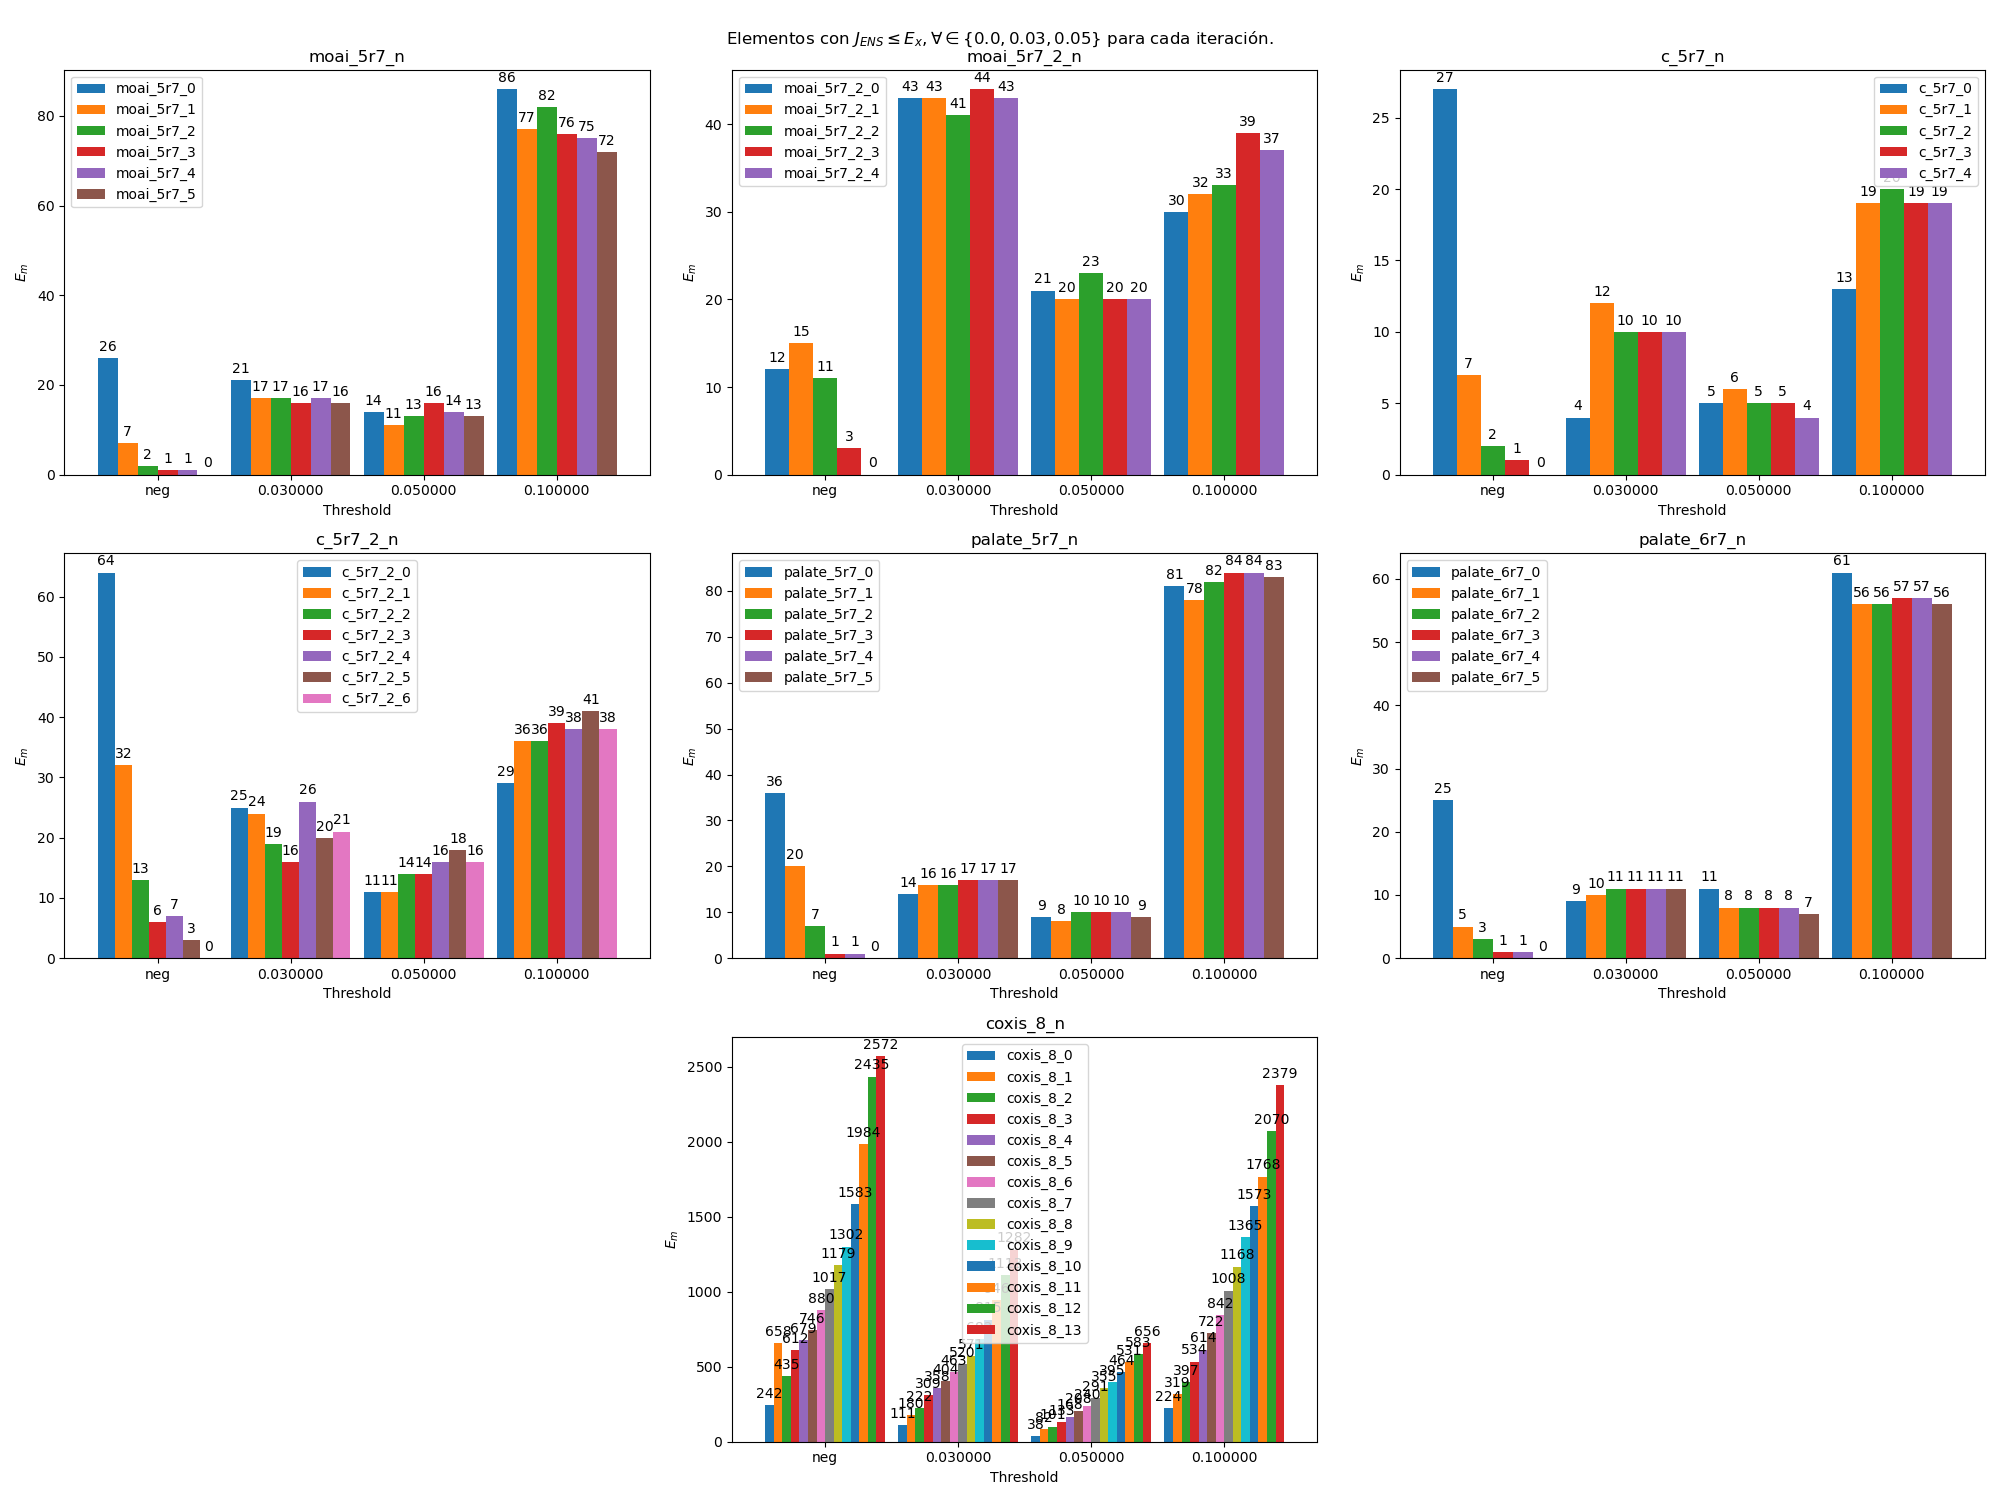
\includegraphics[width=0.75\paperheight, angle=90, origin=c]{figures/analysis/fit_all_bar.png}
	\end{subfigure}
	\caption{ Histograma agrupado por intervalo para todos los casos. }
	Fuente: Elaboración propia.
	\label{fig:fit_all_bar}
\end{figure}

Se puede ver como en la mayoría de los casos válidos, se mantiene constante o varía levemente considerando el orden de magnitud de los Elementos que componen las mallas.



Para la malla del Moai 1 con threshold $0$, \autoref{fig:bar_moai_all}, que contiene $693$ \elements{}, el efecto en cadena generá un delta positivo para el mejoramiento de la malla de aproximadamente $14$ \elements{} en el intervalo $E^{0.05}_{1}$ entre las iteraciones 0 y 5, que decae de $86$ a $72$ \elements{}, es decir, app el $2\%$ de la cantidad de \elements{} de la malla.

Para la malla del Moai 2 con threshold $0$, el efecto generará un delta negativo para el mejoramiento de app $9$ \elements{} en el intervalo $E^{0.05}_{1}$ entre las iteraciones 0 y 3, app el $1.3\%$ de los \elements{} de la malla.  Pero, si nos fijamos el las mismas iteraciones 0 y 3, en los Octantes Objetivo, que serían los \elements{} Inválidos, el delta es positivo para el mejoramiento, disminuyendo drásticamente en la iteración $3$, pasando de $12$ \elements{} en la iteración 0 a $3$ \elements{} en la iteración $3$, algo muy similar al delta del intervalo $E^{0.05}_{1}$.

\begin{figure}[!ht]
	\centering
	\begin{subfigure}[t]{1.0\textwidth}
		\includegraphics[width=0.75\paperheight, angle=90, origin=c]{figures/analysis/moai_bar_all.png}
	\end{subfigure}
	\caption{ Histograma agrupado por intervalo para los dos casos de la malla Moai. }
	Fuente: Elaboración propia.
	\label{fig:bar_moai_all}
\end{figure}

\begin{figure}[!ht]
	\centering
	\begin{subfigure}[t]{1.0\textwidth}
		\includegraphics[width=0.75\paperheight, angle=90, origin=c]{figures/analysis/cortex_bar_all.png}
	\end{subfigure}
	\caption{ Histograma agrupado por intervalo para los dos casos de la malla Corteza.  }
	Fuente: Elaboración propia.
	\label{fig:bar_cortex_all}
\end{figure}


\begin{figure}[!ht]
	\centering
	\begin{subfigure}[t]{1.0\textwidth}
		\includegraphics[width=0.75\paperheight, angle=90, origin=c]{figures/analysis/cortex_bar_all.png}
	\end{subfigure}
	\caption{ Histograma agrupado por intervalo para los dos casos de la malla Paladar.  }
	Fuente: Elaboración propia.
	\label{fig:bar_palate_all}
\end{figure}

\begin{figure}[!ht]
\centering
\begin{subfigure}[t]{1.0\textwidth}
	\includegraphics[width=0.75\paperheight, angle=90, origin=c]{figures/analysis/coxis_bar_all.png}
\end{subfigure}
\caption{ Histograma agrupado por intervalo para los dos casos de la malla Coxis.  }
Fuente: Elaboración propia.
\label{fig:bar_coxis_all}
\end{figure}

Un caso similar, es el de la Corteza 1 para threshold $0$, \autoref{fig:bar_cortex_all}, que en las iteraciones 0 y 5, presenta un delta negativo para el mejoramiento de app $11$ \elements{} en el $E^{0.05}_{1}$, pero en el intervalo  $E^{-\infty}_{0}$ el delta es positivo para el mejoramiento, reduciendo la cantidad de \elements{} Inválidos de $64$ a $3$, casi $5$ veces la cantidad de \elements{} que aumentaron en el intervalo  $E^{0.05}_{1}$. 

Con lo anterior, se puede determinar que muy probablemente los \elements{} mejorados se distribuyen en los intervalos de calidad superiores, incluso cuando se utilizan threshold mayores a $0$, es muy difícil que la calidad en los intervalos inferiores al threshold aumenten su frecuencia de \elements{}, es decir, que los \elements{} empeoren su calidad.


%\breakpoint{ FIN 11-08-2024}
%
%\breakpoint{ INICIO 18-08-2024 }



\subsubsection{ Análisis de calidad frente al Algoritmo de proyección de nodos.}

Para analizar la calidad de las mallas generadas por el algoritmo propuesto en este estudio, se utilizará el estándar fijado en el proceso de validación en \cite{daines2018repairing}, es decir, se utilizarán los tres tipos de refinamientos que soporta el algoritmo, general, local y superficie. Se definirán diferentes regiones de interés (ROI) mostradas en \autoref{fig:regions_all}, respecto a dichas regiones se realizará una homologación, por tanto, los resultados no serán comparables con total precisión. Para reducir la cantidad de iteraciones generadas por el efecto dominó, se utilizará el mismo criterio, un $RL = n$ en la ROI, un $RL = n - 1$ en la superficie de $\Omega$ y un $RL = n - 2$ en el resto de la malla. Se denominará ``cortex\_ref\_reg'' a las instancias, dónde $ref$ es el $RL$ usado por el ROI, y $reg$ el indice identificador de las regiones de interés. En este caso, se utilizará $RL=5$ para las $regiones$, $RL=4$ para la superficie y $RL=3$ para todo el resto. Se definió un máximo de 20 iteraciones, debido al comportamiento inestable que presentaban algunas iteraciones cuando quedaba sólo un \octant{} por refinar.

\begin{figure}[H]
	\centering
	\begin{subfigure}[t]{0.8\textwidth}
		\includegraphics[width=1.0\textwidth]{figures/validation/regions_daines.png}
		\caption{Regiones definidas por \cite{daines2018repairing}.}
	\end{subfigure}
	\begin{subfigure}[t]{1.0\textwidth}
		\includegraphics[width=1.0\textwidth]{figures/validation/regions_pdonoso.png}
		\caption{Regiones homologadas.}
	\end{subfigure}
	\caption{ Regiones de interés usados en instancias de corteza. De izquierda a derecha se identificarán como Región 0 a 6. En (a) se encuentra la referencia utilizada en \cite{daines2018repairing}, en (b) homologadas en la práctica.}
	Fuente: Elaboración propia.
	\label{fig:regions_all}
\end{figure}

El resultado se presenta en \autoref{table:cortex_validation}. Para cada instancia, se disponen cinco filas con la distribución de la calidad de los \elements{}. En la primera fila se muestra la distribución del algoritmo original. Luego, las 2 filas siguientes representan a las pruebas realizadas con algoritmo de proyección de nodos con threshold $0.03$ y $0.05$, respectivamente y finalmente las 2 filas siguientes corresponden a las pruebas realizadas por el algoritmo propuesto con los mismos threshold definidos para el algoritmo de proyección de nodos.

En la primera columna se muestra el $J_{ENS}$ mínimo de la malla generada, es decir, el \element{} de peor calidad, luego se muestran las frecuencias de los \elements{} que pertenecen a dicho intervalo de calidad desde \elements{} de calidad negativa hasta $J_{ENS} = 0.2$. Al final, la última columna nos muestra la cantidad total de \elements{} de la malla.


\begin{table}[H]
	\scriptsize 
	\centering
	\begin{tabular}{lc cc cc cc c}
		\hline
		Instance & $J_{ENS}min$ & Inv & [0, 0.03[ & [0.03, 0.05[ & [0.05, 0.1[ & [0.1, 0.15[ & [0.15, 0.2[ & $Total$ \\
		\hline
		\texttt{cortex\_5\_0} & -0.009743 & 1 & 8 & 8 & 14 & 35 & 31 & 12895 \\
		& 0.037720 & 0 & 0 & 7 & 9 & 34 & 38 & 12891 \\
		& 0.053261 & 0 & 0 & 0 & 7 & 35 & 42 & 12875 \\
		& 0.039391 & 0 & 0 & 3 & 13 & 20 & 32 & 13322 \\
	 	& 0.051298 & 0 & 0 & 0 & 12 & 21 & 33 & 13704 \\
		\hline
		\texttt{cortex\_5\_1} & -0.000639 & 1 & 7 & 2 & 9 & 18 & 29 & 12005 \\
		& 0.041439 & 0 & 0 & 2 & 9 & 18 & 24 & 11983 \\
		& 0.058775 & 0 & 0 & 0 & 9 & 18 & 25  & 11988 \\
		& 0.031648 & 0 & 0 & 3 & 8 & 24 & 49 & 15686 \\
		& 0.062543 & 0 & 0 & 0 & 13 & 25 & 52 & 15828 \\
		\hline
		\texttt{cortex\_5\_2} & 0.002585 & 0 & 3 & 2 & 13 & 22 & 36 & 8329 \\
		& 0.030672 & 0 & 0 & 4 & 13 & 21 & 36 & 8327 \\
		& 0.059482 & 0 & 0 & 0 & 13 & 22 & 38 & 8290 \\
		& 0.031067 & 0 & 0 & 3 & 11 & 19 & 40 & 8448 \\
		& 0.058946 & 0 & 0 & 0 & 12 & 19 & 43 & 8515 \\
		\hline
		\texttt{cortex\_5\_3} & -0.999649 & 3 & 0 & 1 & 11 & 44 & 86 & 11902 \\
		& 0.041507 & 0 & 0 & 2 & 12 & 47 & 79 & 11903 \\
		& 0.000000 & 0 & 2 & 2 & 22 & 48 & 84 & 11886 \\
		& 0.032822 & 0 & 0 & 1 & 14 & 27 & 100 & 14340 \\
		& 0.051203 & 0 & 0 & 0 & 15 & 28 & 103 & 14378 \\
		\hline
		\texttt{cortex\_5\_4} & -0.222353 & 2 & 2 & 1 & 9 & 34 & 63 & 18513 \\
		& 0.042440 & 0 & 0 & 1 & 7 & 32 & 64 & 18506 \\
		& 0.056449 & 0 & 0 & 0 & 7 & 31 & 67 & 18495 \\
		& 0.055131 & 0 & 0 & 0 & 5 & 16 & 50 & 18661 \\
		& 0.055131 & 0 & 0 & 0 & 5 & 16 & 50 & 18661 \\
		\hline
		\texttt{cortex\_5\_5} & -0.100899 & 2 & 2 & 0 & 8 & 30 & 55 & 9866 \\
		& 0.072093 & 0 & 0 & 3 & 9 & 33 & 57 & 9871 \\
		& 0.072093 & 0 & 0 & 0 & 7 & 33 & 57 & 9871 \\
		& 0.038194 & 0 & 0 & 2 & 8 & 15 & 95 & 13248 \\
		& 0.050810 & 0 & 0 & 0 & 8 & 14 & 94 & 13294 \\
 		\hline
		\texttt{cortex\_5\_6} & -0.491747 & 9 & 0 & 0 & 2 & 47 & 71 & 9635 \\
		& -0.981794 & 11 & 1 & 3 & 19 & 55 & 79 & 9599 \\
		& -0.981794 & 11 & 1 & 3 & 19 & 55 & 79 & 9599 \\
		& 0.038194 & 0 & 0 & 1 & 3 & 10 & 64 & 10076 \\
		& 0.007059 & 0 & 0 & 0 & 3 & 10 & 64 & 10257 \\
		\hline
		\multicolumn{7}{l}{ $J_{ENS}min$: Jens mínimo, el \element{} de peor calidad.} \\
		\multicolumn{7}{l}{ $Inv$: \elements{} con calidad menor a $0$.} \\
		\multicolumn{7}{l}{ $Total$: Cantidad de \elements{} que componen la malla.} \\
		\multicolumn{7}{l}{ En cada instancia: }\\
		\multicolumn{7}{l}{\hspace{1em} - Primera fila: Algoritmo Original.}\\
		\multicolumn{7}{l}{\hspace{1em} - Segunda fila: Algoritmo de proyección de nodos con threshold $0.03$.}\\
		\multicolumn{7}{l}{\hspace{1em} - Tercera fila: Algoritmo de proyección de nodos con threshold $0.05$.}\\
		\multicolumn{7}{l}{\hspace{1em} - Cuarta fila: Algoritmo de refinamiento de octantes con threshold $0.03$.}\\
		\multicolumn{7}{l}{\hspace{1em} - Quinta fila: Algoritmo de refinamiento de octantes con threshold $0.05$.}
	\end{tabular}
	\caption{Comparación de calidad de los resultados entre los algoritmos original, proyección de nodos y refinamiento de octantes. }
	\label{table:cortex_validation}
\end{table}


\vspace{4pt}
\hrule
\vspace{4pt}

Se añadió el algoritmo propuesto a la comparación de tiempo y calidad realizada por \cite{daines2018repairing}, en la \autoref{table:cortex_qt}, se evidencia, al igual que en la tabla referenciada anteriormente, las 7 regiones estudiadas para la corteza cerebral, en cada fila que representa a cada instancia, se encuentran tres filas, la primera muestra la calidad y tiempo de ejecución de la instancia con el algoritmo original, en la segunda fila se utiliza el algoritmo de proyección de nodos y en la tercera fila el algoritmo propuesto.

Para medir la calidad, se utilizó el $J_{ENS}$ mínimo de todos los \elements{} de la malla resultante y para el tiempo, medido en segundos, se definirá como el tiempo por iteración $\frac{T}{it}$, considerado como el tiempo promedio de cada iteración, esta expresión no incluye la primera iteración porque se considera aproximadamente similar al tiempo de ejecución del algoritmo original, se define formalmente en \autoref{eq:tit}.

 
\begin{equation} \label{eq:tit}
	\begin{aligned}
		\frac{T}{it} &= \frac{TO - TP}{TP - 1}
	\end{aligned}
\end{equation}
 
 
\begin{table}[H]
	\centering
	\begin{tabular}{|l|c|c|c|c|}
		\hline
		Instance & $J_{ENS}min$ & T [s] & It & T/it [s] \\ \hline
			cortex\_5\_0 & -0.009743 & 2.312 & - & - \\
			&  0.037720 & 2.917 & 2 & 0.605 \\
			&  0.039391 & 2.735 & 4 & 0.683 \\
		\hline
			cortex\_5\_1 & -0.000639 & 2.111 & - & - \\
			& 0.041439 & 2.698 & 2 & 0.587 \\ 
			& 0.031648 & 3.879 & 5 & 0.775 \\
		\hline
			cortex\_5\_2 & 0.002585 & 1.776 & - & - \\
			& 0.030672 & 2.247 & 2 & 0.471 \\ 
			& 0.031067 & 1.015 & 2 & 0.507 \\
		\hline
			cortex\_5\_3 & -0.999649 & 2.060 & - & - \\
			& 0.041507 & 2.595 & 2 & 0.535 \\ 
			& 0.032822 & 2.655 & 4 & 0.663 \\
		\hline
			cortex\_5\_4 & -0.222353 & 2.819 & - & - \\
			& 0.042440 & 3.637 & 2 & 0.818 \\ 
			& 0.055131 & 1.788 & 2 & 0.894 \\
		\hline
			cortex\_5\_5 & -0.100899 & 1.813 & - & - \\
			& 0.072093 & 2.275 & 2 & 0.462 \\ 
			& 0.038194 & 5.743 & 9 & 0.638 \\
		\hline
			cortex\_5\_6 & -0.491747 & 1.800 & - & - \\
			& -0.981794 & 3.637 & 5 & 0.459 \\ 
			& 0.038194 & 4.167 & 8 & 0.520 \\
		\hline
		\multicolumn{5}{l}{ $J_{ENS}$: Jens mínimo, el \element{} de peor calidad.} \\
		\multicolumn{5}{l}{ $T$: Tiempo total de la ejecución del algoritmo.} \\
		\multicolumn{5}{l}{ $It$: Cantidad de iteraciones realizadas.}
	\end{tabular}
	\caption{Comparación en tiempo y calidad entre los algoritmos original, proyección de nodos y refinamiento de octantes, con threshold $0.03$.}
	\label{table:cortex_qt}
\end{table}

Al analizar los resultados de calidad y tiempo, se puede notar que el tiempo total de las ejecuciones de los casos de prueba, aumentan considerablemente, incluso en algunos casos aumentando un $100\%$ del tiempo de la ejecución del algoritmo de proyección de nodos, pero, si bien el tiempo total aumenta, el tiempo por iteración, se mantiene relativamente similar.

Este algoritmo y el propuesto para proyectar los nodos presentan la misma complejidad computacional $O(n\cdot2M)$, siendo $M$ la cantidad de nodos y $n$ la cantidad de iteraciones, por tanto, ambos debiesen presentar tiempos por iteración lineales y similares. Evidencia de lo anterior, es la similitud entre estos factores para ambos algoritmos, con una variación del orden de las décimas de segundo por iteración.

Por otra parte, el $J_{ENS}min$ para el algoritmo propuesto se mantiene más cercano al threshold que el algoritmo de proyección de nodos, esto podría interpretarse como un efecto en la vecindad por parte de este último algoritmo, no así el propuesto, que en caso de que la calidad de los \elements{} no presente calidad inferior a la cota, entonces no aplicará refinamiento, es decir, priorizará mantener la calidad existente mientras no existan \elements{} de peor calidad que el threshold.


%  TODO: presentar analisis breve de las fallas en la malla coxis, propuestas de posibles problemáticas y soluciones viables.